\documentclass{ijuc}
\usepackage[pdftex]{graphics}
\usepackage{graphicx}
\usepackage{amssymb}
\usepackage{hyperref}
\usepackage[normalem]{ulem}
\usepackage{amsmath}
\usepackage{siunitx}

\begin{document}

\title{Combinatorial approach to counting equivalence classes in 1D and 2D cellular automata}
\author{Iztok Jeras\inst{1}\email{iztok.jeras@rattus.info}}
\institute{Faculty of Computer and Information Science, University of Ljubljana, Slovenia}
\def\received{Received 17 December 2004; In final form 1 April 2005}

\maketitle

\begin{abstract}
There is much more theoretical research on 1D cellular automata compared to 2D.
While not the only reason one of the arguments given is that the number of
available rules for a common 2D neighborhood is too large for a comprehensive
analysis. This issue can be mitigated by focusing on the smallest 2D neighborhoods
(trid and quad) and by grouping rules into equivalence classes. This article
gives an algebraic combinatorial solution to counting equivalence classes.
\end{abstract}

\keywords{cellular automata, combinatorics, equivalence classes, congruence operations}

\section{Introduction}

The focus of theoretical research is usually the simplest possible version of a system.
For 1D CA elementary rules are the simplest which exhibit not trivial behavior. Rule
equivalence has been used by many authors to organize 256 elementary CA rules into 88
equivalence classes. Representative rules from each class were then observed and described.
This approach found the most interesting rules which were then further analyzed. Rule 110
is a good example.

The same approach was never applied to 2D CA. For example most studied 2D rule is Game of Life.
It is based on a Moore neighborhood is binary cells. There are $2^{2^9}=2^512$ possible rules,
too many for a comprehensive analysis of the entire rule space. The von Neumann neighborhood
with $2^{2^5}=2^32$ rules is still impractical, and there is no rule with this neighborhood on
a binary lattice, which would receive as much attention as Game of Life. While this two
neighborhoods were the focus of 2D CA research till recently, there are two simpler neighborhoods
named quad and trid which were popularized by Tommaso Toffoli only in 2008 using the QUAD prize competition.
The aim of the QUAD prize was to find a computation-universal 2-state cellular automaton on a 2-dimensional,
2×2-neighborhood. Edward Powley proved computational universality on an even smaller neighborhood, the trid.

The focus of my CA research are preimages. On 1D CA de Bruijn diagrams are the main tool
used for this research. The size of this diagrams depends on the size of the rue space.
While once the algorithms for calculating preimages are known, the ability to compute
them is only limited by computer memory, the research of such algorithms usually requires
the ability of the researcher to model such problems with mathematical notations like
graphs and matrices. Only with 2D neighborhoods as small as quad and trid such representations
become small enough for theoretical analysis with the help of visual representations.

The purpose of this article is to calculate the number of equivalence classes for a few small
neighborhoods on a binary lattice (2D and 3D). The number of interesting rules can be further
reduced by removing rules which can be represented with a smaller neighborhood. This are rules
where one of the neighbors is not used in the local transition function, and higher order rules,
those that can be represented with multiple steps of a smaller neighborhood rule.

??? Most research on CA was recently done by Hidenosuke Nishio \cite{DBLP:journals/jca/Nishio12},
\cite{DBLP:journals/fuin/Nishio10}, \cite{DBLP:conf/ncma/Nishio09}, \cite{DBLP:conf/automata/NishioW08}.

Tommaso Toffoli
\url{http://uncomp.uwe.ac.uk/automata2008/files/quad.pdf}

Edward Powley
\url{http://uncomp.uwe.ac.uk/automata2008/files/quadprize_powley.pdf}

\section{Formalization}

I will skip the full CA formalization and will focus on aspects observed in this article.
What needs to be defined is the number of states of a cell, symmetries of the underlying lattice,
the neighborhood shape, and the rule value.

Each cell \(c\) can be in one of \(k\) states, which are numbered starting with 0.
There are \(k!\) permutations of the state set.
\[ c \in {0, 1, ..., k-1} \]
\[ \vert G^{per} \vert = k! \]

The underlaying lattice can have one or more dimensions. In 1D only reflection symmetry exists,
while in 2D there is also a 3, 4 or 6 fold rotation symmetry. 3D or lattices with even more
dimensions are not discussed here, although the same principles can be applied there.

Regardless of the underlying lattice only two reflections, unchanged and mirrored.
\[ G^{ref} = (if, ref) \]
\[ \vert G^{ref} \vert = 2 \]

The number of rotations depends on the underlying lattice and is discussed for each neighborhood shape.

The neighborhood is defined by the number of cells \(m\) and its shape.
Only the trid and quad 2D neighborhoods will be discussed.
The neighborhood value is an ordered list of cell values. There are \(k^m\) possible neighborhood values.
\[ n = (c_0, c_1, ..., c_{m-1}) \]

The local transition function maps a neighborhood state into the next state of a cell.
\[ f(n) = c_n \]
It is defined by as many cell values as there are neighborhood values.
\[ r = (f(0), f(1), ..., f(k^m)) \]

The relative position between a call and its neighborhood is not relevant for this article.
But to understand the symmetries it is important to formalize the positions of cells inside a neighborhood.

\subsection{1D}

For 1D CA cells inside a neighborhood are numbered from left to right (see Figure \ref{fig-linear}).

\begin{figure}
\begin{center}
\scalebox{0.3}{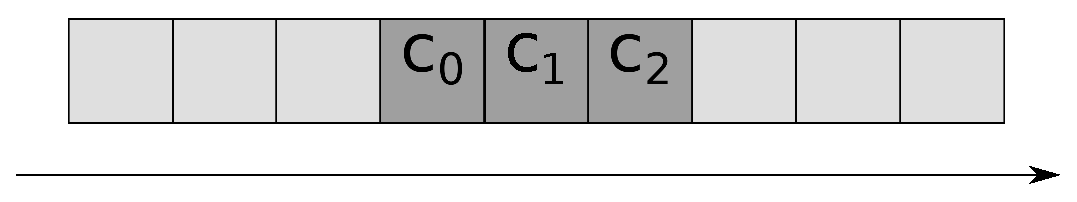
\includegraphics{linear.eps}}
\end{center}
\caption{Elementary neighborhood on a linear lattice.}
\label{fig-linear}
\end{figure}

\subsection{2D trid}

Due to symmetries all enumerations of neighborhood cells for trid are equivalent.
Here enumeration starts in the left bottom corner and continues in a counter clockwise loop (see Figure \ref{fig-trid}).

\begin{figure}
\begin{center}
\scalebox{0.3}{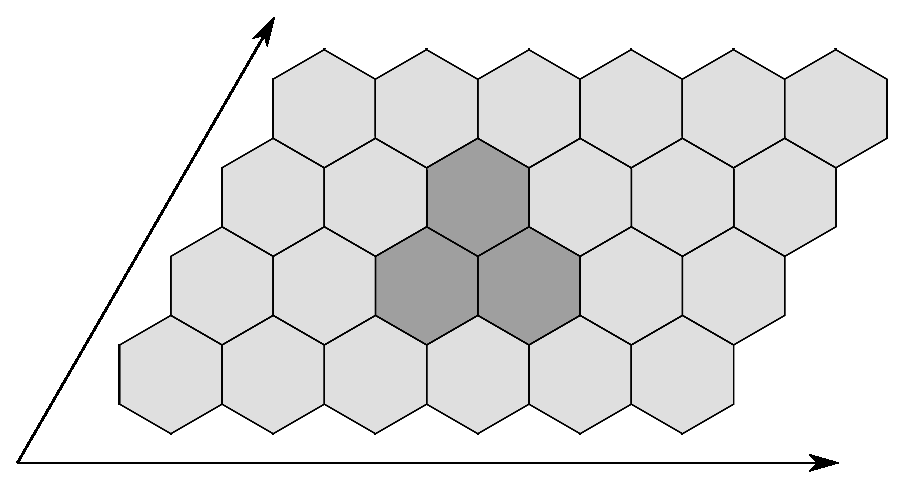
\includegraphics{trid.eps}}
\end{center}
\caption{Trid neighborhood on a hexagonal lattice.}
\label{fig-trid}
\end{figure}

\subsection{2D quad}

To simplify the representation of rotations enumeration for quad also starts
in the left bottom corner and continues in a counter clockwise loop (see Figure \ref{fig-quad}).

\begin{figure}
\begin{center}
\scalebox{0.3}{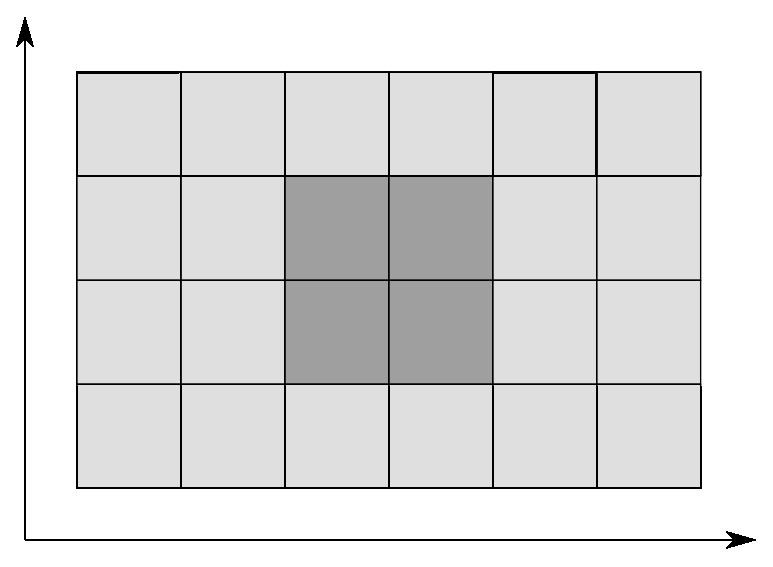
\includegraphics{quad.eps}}
\end{center}
\caption{Quad neighborhood on a square lattice.}
\label{fig-quad}
\end{figure}

\section{Definition of Equivalence}

Two rules \( r_{A}, r_{B} \) are equivalent, if a transformation \(\varphi\) for the CA state exists, such that each CA
current-next state pair \( (C^{t}, C^{t+1}) \) for the current rule gets transformed into a current-next state pair
for the other rule.

\[ r_{A} \sim r_{B}  \Leftrightarrow  \forall C_{B}=\varphi(C_{A}) : F_{B}=\varphi(F_{A}) : F_{A}(C_{A}^{t}) = C_{A}^{t+1}, F_{B}(C_{B}^{t}) = C_{B}^{t+1} : C_{A}^{t+1} = C_{B}^{t+1} \]

State transition graphs for equivalent rules are of the same shape, and a transformation exists
which maps each state in one graph to a state at the same position in the graph for the other rule.

There are generalizations to this definition. For example a rule and it second order rule can be thought as equivalent.
(rule performing the same global transition in one step as the original rule achieves in two steps.

\section{1D problem}

Equivalence groups for elementary CA are long known. What is missing is a general algebraic solution.

\subsection{Symmetries}

There is a set of known symmetries or congruence operations on a given CA state.
For 1D CA this are reflection and permutation.

Reflection:

\[ G_{ref} = (id, ref) \]
\[ \vert G_{ref} \vert = 2 \]

Permutation:

\[ G_{per} = (id, per) \]
\[ \vert G_{per} \vert = k! \]

\subsection{Counting neighborhood values}

The set of all distinct neighborhood values $\mathbb{M}$ for a given neighborhood size $n$ and
number of cell states $k$ is:

\[ M = \left\{ m : \right\} \]
\[ \vert \mathbb{M} \vert = k^n \]

Neighborhood values can be organized into subsets depending on their invariance to congruence operations.

There are neighborhood values which are invariant to reflection. This are neighborhoods for which the
left half is the mirror is the mirror image of the right half. There are as many such neighborhood
values as there are possible values for a half sized neighborhood. For odd neighborhood sizes the middle
cell is always a mirror image of itself.

\[ \mathbb{M}_\mathrm{ref} = \left\{ \forall n \in \mathbb{M} : \phi_\mathrm{ref}(n) = n \right\} \]
\[ \vert \mathbb{M}_\mathrm{ref} \vert = \left\{ 
  \begin{array}{ll}
    {k^{m/2+1}} & \quad \textrm{if $m$ is odd }\\
    {k^{m/2  }} & \quad \textrm{if $m$ is even}
  \end{array} \right.
\]

There are no neighborhood values which are invariant to permutation.

\[ \mathbb{M}_\mathrm{per} = \left\{ \forall n \in \mathbb{M} : \phi_\mathrm{per}(n) = n \right\} = \varnothing \]
\[ \vert \mathbb{M}_\mathrm{per} \vert = 0 \]

There are neighborhood values which are invariant after both reflection and permutation have been applied.

\[ \mathbb{M}_\mathrm{ref,per} = \left\{ \forall n \in \mathbb{M} : \phi_\mathrm{per}(\phi_\mathrm{ref}(n)) = n \right\} \]
\[ \vert \mathbb{M}_\mathrm{ref,per} \vert = \left\{ 
  \begin{array}{ll}
    {0        } & \quad \textrm{if $m$ is odd }\\
    {k^{m/2  }} & \quad \textrm{if $m$ is even}
  \end{array} \right.
\]

\subsection{Counting rules}

Number of all rules \(\vert R \vert\):

\[ \vert R \vert = k^{\vert M \vert} = k^{k^n} \]

Rules which are invariant to reflection. The calculation is based on the number of
reflection invariant neighborhood values. The local transition function can take any
value for reflection invariant neighborhood values \(M^\mathrm{ref}\) while for the
rest \(M  \setminus M^\mathrm{ref}\) the same value must be used
for the the neighborhood value and its reflection.

\[ R^\mathrm{ref} = \left\{ \forall r \in R : \mathrm{ref}(r) = r \right\} \]
\[ \vert R^\mathrm{ref} \vert = k^{ \vert M^\mathrm{ref} \vert + \frac{\vert M \vert - \vert M^\mathrm{ref} \vert}{2} } = k^{ \frac{\vert M \vert + \vert M^\mathrm{ref} \vert}{2} } \]
\[ \vert R^\mathrm{ref} \vert = \left\{ 
  \begin{array}{ll}
    k^{\frac{k^m + k^{m/2+1}}{2}} & \quad \textrm{if $m$ is odd }\\
    k^{\frac{k^m + k^{m/2  }}{2}} & \quad \textrm{if $m$ is even}
  \end{array} \right.
\]

Rules which are invariant to permutation.

\[ R^\mathrm{per} = \left\{ \forall r \in R : \mathrm{per}(r) = r \right\} \]
\[ \vert R^\mathrm{per} \vert = k^{\vert M \vert / k} \]

Rules which are invariant to reflection and permutation applied at the same time.
First permutation limits free variables to \(k^{\vert M \vert / k}\), then reflection
limits them further by allowing a single free variable for all non reflective neighborhood values.
TODO: check this for correctness.

\[ R^\mathrm{ref \& per} = \left\{ \forall r \in R : \mathrm{per}(\mathrm{ref}(r)) = r \right\} \]
k=2
\[ \vert R^\mathrm{ref \& per} \vert = \left\{ 
  \begin{array}{ll}
    k^{1 + 1} & \quad \textrm{if $m$ is odd }\\
    k^{k + 1} & \quad \textrm{if $m$ is even}
  \end{array} \right.
\]
\subsection{Counting equivalence classes}

\url{https://en.wikipedia.org/wiki/Burnside%27s_lemma}

Burnside's lemma is used to count equivalence classes:

\[ |X/G| = \frac{1}{|G|}\sum_{g \in G}|X^g| \]

where G is 
\[ G_{ref} = (id, ref) \]
\[ G_{per} = (id, per) \]
\[ G = G_{ref} \times G_{per} = (id, ref, per, ref \& per) \]

\[ |X/G| = \frac{1}{2 \times k!} ( R + R^{ref} + (|G^{per}|-1)*(R^{per} + R^{per \& ref}) ) \]

Result for elementary CA (\(k=2\), \(n=3\))
\[ |X/G| = \frac{1}{4} (2^8 + 2^6 + 2^4 + 2^4) = 88 \]

\section{2D problem}

\subsection{Symmetries}

In addition to reflection and permutation symmetries already present in 1D CA,
2D CA also exhibit rotation symmetry. The number of available rotations depends
on the underlaying lattice.

3-fold: trid
4-fold: quad, Moore, von Neumann neighborhood
6-fold: hexagonal lattice

\[ G_{rot} = (id, rot) \]
\[ \vert G_{per} \vert =  \]

\subsection{Trid}

\begin{table}
\begin{center}
\begin{tabular}{cc|cc|cc|cc}
\multicolumn{2}{c|}{} & \multicolumn{2}{c|}{per} & \multicolumn{2}{c|}{ref} & \multicolumn{2}{c}{per,ref} \\ \hline
000 & 0               &       111  &       7  0  &       000  &       0     &       111  &       7  0     \\
001 & 1               &       110  &       6  1  &       100  &       4  1  &       011  &       3  1     \\
010 & 2               &       101  &       5  2  &       010  &       2     &       101  &       5  2     \\
011 & 3               &       100  &       4  3  &       110  &       6  3  & \sout{001} & \sout{1} 3     \\
100 & 4               & \sout{011} & \sout{3} 4  & \sout{001} & \sout{1} 4  &       110  &       6  4     \\
101 & 5               & \sout{010} & \sout{2} 5  &       101  &       5     & \sout{010} & \sout{2} 5     \\
110 & 6               & \sout{001} & \sout{1} 6  & \sout{011} & \sout{3} 6  & \sout{100} & \sout{4} 6     \\
111 & 7               & \sout{000} & \sout{0} 7  &       111  &       7     & \sout{000} & \sout{0} 7     \\
\end{tabular}
\begin{tabular}{cc|cc|cc|cc}
\multicolumn{2}{c|}{rot1} & \multicolumn{2}{c|}{rot1,per} & \multicolumn{2}{c|}{rot1,ref} & \multicolumn{2}{c}{rot1,per,ref} \\ \hline
      000  &       0      &       111  &       7  0         &       000  &       0          &       111  &       7  0          \\
\sout{010} & \sout{2} 1 4 &       101  &       5  1 4 3 2 6 &       001  &       1          &       110  &       6  1          \\
\sout{100} & \sout{4} 2 1 & \sout{011} & \sout{3} 2 ...     &       100  &       4  2       &       011  &       3  2          \\
      110  &       6  3 5 & \sout{001} & \sout{1} 3 ...     & \sout{101} & \sout{5} 3       & \sout{010} & \sout{2} 3          \\
      001  &       1  4 2 & \sout{110} & \sout{6} 4 ...     & \sout{010} & \sout{2} 4       &       101  &       5  4          \\
\sout{011} & \sout{3} 5 6 & \sout{100} & \sout{4} 5 ...     &       011  &       3  5       & \sout{100} & \sout{4} 5          \\
\sout{101} & \sout{5} 6 3 & \sout{010} & \sout{2} 6 ...     &       110  &       6          & \sout{001} & \sout{1} 6          \\
      111  &       7      & \sout{000} & \sout{0} 7 ...     &       111  &       7          & \sout{000} & \sout{0} 7          \\
\end{tabular}
\begin{tabular}{cc|cc|cc|cc}
\multicolumn{2}{c|}{rot2} & \multicolumn{2}{c|}{rot2,per} & \multicolumn{2}{c|}{rot2,ref} & \multicolumn{2}{c}{rot2,per,ref} \\ \hline
      000  &       0      &       111  &       7  0         &       000  &       0          &       111  &       7  0          \\
\sout{100} & \sout{4} 1 2 &       011  &       3  1 2 6 4 5 &       010  &       2  1       &       101  &       5  1          \\
\sout{001} & \sout{1} 2 4 & \sout{110} & \sout{6} 2 ...     & \sout{001} & \sout{1} 2       &       110  &       6  2          \\
      101  &       5  3 6 & \sout{010} & \sout{2} 3 ...     &       011  &       3          &       100  &       4  3          \\
      010  &       2  4 1 & \sout{101} & \sout{5} 4 ...     &       100  &       4          & \sout{011} & \sout{3} 4          \\
\sout{110} & \sout{6} 5 3 & \sout{001} & \sout{1} 5 ...     &       110  & \sout{6} 5       & \sout{001} & \sout{1} 5          \\
\sout{011} & \sout{3} 6 5 & \sout{100} & \sout{4} 6 ...     & \sout{101} &       5  6       & \sout{010} & \sout{2} 6          \\
      111  &       7      & \sout{000} & \sout{0} 7 ...     &       111  &       7          & \sout{000} & \sout{0} 7          \\
\end{tabular}
\end{center}
\caption{My caption}
\label{tbl-trid}
\end{table}

Counter clockwise rotations for \SI{120}{\degree}.
\[ G_{rot} = (id=rot0, rot1, rot2) \]
\[ \vert G_{rot} \vert = 3 \]

\[ G = G_{ref} \times G_{per} \times G_{rot} \]
\[ \vert G \vert = 12 \]

\[ |X/G| = \frac{1}{12} \left( (2^8 + 2^6 + 2^4 + 2^4) + 2 (2^4 + 2^2 + 2^6 + 2^4) \right) = 36 \]
\subsection{Quad}

\begin{table}
\begin{center}
\begin{tabular}{cc|cc|cc|cc}
\multicolumn{2}{c|}{} & \multicolumn{2}{c|}{per} & \multicolumn{2}{c|}{ref} & \multicolumn{2}{c}{per,ref} \\ \hline
0000 & 0              &       1111  &       F  0 &       0000  &       0     &       1111  &       F  0     \\
0001 & 1              &       1110  &       E  1 &       1000  &       8  1  &       0111  &       7  1     \\
0010 & 2              &       1101  &       D  2 &       0100  &       4  2  &       1011  &       B  2     \\
0011 & 3              &       1100  &       C  3 &       1100  &       C  3  &       0011  &       3        \\
0100 & 4              &       1011  &       B  4 & \sout{0010} & \sout{2} 4  &       1101  &       D  4     \\
0101 & 5              &       1010  &       A  5 &       1010  &       A  5  &       0101  &       5        \\
0110 & 6              &       1001  &       9  6 &       0110  &       6  6  &       1001  &       9  6     \\
0111 & 7              &       1000  &       8  7 &       1110  &       E  7  & \sout{0001} & \sout{1} 7     \\
1000 & 8              & \sout{0111} & \sout{7} 8 & \sout{0001} & \sout{1} 8  &       1110  &       E  8     \\
1001 & 9              & \sout{0110} & \sout{6} 9 &       1001  &       9     & \sout{0110} & \sout{6} 9     \\
1010 & A              & \sout{0101} & \sout{5} A & \sout{0101} & \sout{5} A  &       1010  &       A        \\
1011 & B              & \sout{0100} & \sout{4} B &       1101  &       D  B  & \sout{0010} & \sout{2} B     \\
1100 & C              & \sout{0011} & \sout{3} C & \sout{0011} & \sout{3} C  &       1100  &       C        \\
1101 & D              & \sout{0010} & \sout{2} D & \sout{1011} & \sout{B} D  & \sout{0100} & \sout{4} D     \\
1110 & E              & \sout{0001} & \sout{1} E & \sout{0111} & \sout{7} E  & \sout{1000} & \sout{8} E     \\
1111 & F              & \sout{0000} & \sout{0} F &       1111  &       F     & \sout{0000} & \sout{0} F     \\
\end{tabular}
\begin{tabular}{cc|cc|cc|cc}
\multicolumn{2}{c|}{rot1} & \multicolumn{2}{c|}{rot1,per} & \multicolumn{2}{c|}{rot1,ref} & \multicolumn{2}{c}{rot1,per,ref} \\ \hline
0000 & 0              &       1111  &       F  0     &       0000  &       0     &       1111  &       F  0     \\
0010 & 2 1 4 8        &       1101  &       D  1 4 7 &       0001  &       1     &       1110  &       E  1     \\
0100 & 4 2 8 1        &       1011  &       B  2 8 E &       1000  &       8  2  &       0111  &       7  2     \\
0110 & 6 3 C 9        &       1001  &       9  3 C 6 &       1001  &       9  3  &       0110  &       6  3     \\
1000 & 8 4 1 2        &       0111  &       7  4 1 D & \sout{0100} &       4     &       1011  &       B  4     \\
1010 & A 5            &       0101  &       5        &       0101  &       5     &       1010  &       A  5     \\
1100 & C 6 9 3        &       0011  &       3  6 9 C &       1100  &       C  6  &       0011  & \sout{3} 6     \\
1110 & E 7 D B        &       0001  &       1  7 D 4 &       1101  &       D  7  & \sout{0010} & \sout{2} 7     \\
0001 & 1 8 2 4        & \sout{1110} & \sout{E} 8 2 B & \sout{0010} & \sout{2} 8  &       1101  &       D  8     \\
0011 & 3 9 6 C        & \sout{1100} & \sout{C} 9 6 3 &       0011  & \sout{3} 9  & \sout{1100} &       C  9     \\
0101 & 5 A            &       1010  &       A        & \sout{1010} &       A     &       0101  & \sout{5} A     \\
0111 & 7 B E D        & \sout{1000} & \sout{8} B E 2 &       1011  &       B     & \sout{0100} & \sout{4} B     \\
1001 & 9 C 3 6        & \sout{0110} & \sout{6} C 3 9 & \sout{0110} & \sout{6} C  &       1001  & \sout{9} C     \\
1011 & B D 7 E        & \sout{0100} & \sout{4} D 7 1 & \sout{0111} & \sout{7} D  & \sout{1000} & \sout{8} D     \\
1101 & D E B 7        & \sout{0010} & \sout{2} E B 8 & \sout{1110} &       E     & \sout{0001} & \sout{1} E     \\
1111 & F              & \sout{0000} & \sout{0} F     &       1111  &       F     & \sout{0000} & \sout{0} F     \\
\end{tabular}
\end{center}
\caption{My caption}
\label{tbl-quad}
\end{table}

Counter clockwise rotations for \SI{90}{\degree}.
\[ G_{rot} = (id=rot0, rot1, rot2, rot3) \]
\[ \vert G_{rot} \vert = 4 \]

\[ G = G_{ref} \times G_{per} \times G_{rot} \]
\[ \vert G \vert = 16 \]

\[ |X/G| = \frac{1}{16} \left( (2^{16} + 2^8 + 2^{10} + 2^{10}) + 3 (2^{2+2/2+12/4} + 2^{2+2/2+12/4} + 2^{8/2}) \right) = ... \]
\[ |X/G| = \frac{1}{16} \left( (2^{16} + 2^8 + 2^{10} + 2^{10}) + 3 (2^{2+1+3}      + 2^{2+1+3}      + 2^{4}  ) \right) = ... \]
\[ |X/G| = \frac{1}{16} \left( (2^{16} + 2^8 + 2^{10} + 2^{10}) + 3 (2^{6}          + 2^{8}          + 2^{4}  ) \right) = ... \]
\[ |X/G| =              \left( (2^{12} + 2^4 + 2^6 + 2^6) + 3 (2^2 + 2^8 + 2^0) \right) = ... \]
\[ |X/G| =              \left( (2^{12} + 16 + 128) + 3 (4 + 156 + 1) + \right) = 4723 \]

\section{Conclusion}

With elementary cellular automata the approach was to observe the evolution of
each rule and to further study the ones which exhibit interesting behavior.
A similar approach can be taken with 2D trid and quad. With an appropriate filter
this evolutions could be made into a video or a 3D image. An example filter would
convert each 3×3 neighborhood pattern probabilities into a color palette. For trid
a single person could do the review, while for quad crowd-sourcing could be used.

I hope will help further theoretical research into 2D CA.

\bibliography{equivalence}

\appendix 

\end{document}
